\documentclass[thmcnt=section, 12pt, color=cyan]{my-elegantbook}

% index page
\usepackage{imakeidx}
\makeindex[columns=2, intoc, options=-s index_style.ist]

% title and author
\title{Graph Theory}
\author{Isaac FEI}

% reference file
\addbibresource{Graph Theory.bib} 

% image of the book cover
\cover{cover2}

\begin{document}

% Print title and cover page
\maketitle

%--------
% preface
%--------

\frontmatter
\section*{Preface}

I mainly refer to \parencite{bondyGraphTheoryApplications1976}.


%------------------------------

% Print table of contents
\tableofcontents
\mainmatter

%-------------------------------
% main document starts from here
%-------------------------------

%==============================

\chapter{Basic Concepts of Graphs}

%------------------------------

\section{Isomorphism}

Two graphs $G$ and $H$ are identical, written as $G = H$, if all their components are the same, that is, $V(G) = V(H)$, $E(G) = E(H)$ and $\psi_G = \psi_H$. Identical graphs of course share the same properties. However, a graph $H$ does not necessarily have to be exactly $G$ to preserve all its properties. The labels of the vertices and edges are immaterial.

\begin{definition}
    Two graphs $G$ and $H$ are said to be isomorphic, written as $G \cong H$, if there exist bijections $\theta: V(G) \to V(H)$ and $\phi: E(G) \to E(H)$ such that 
    \begin{align}
        \psi_G(e) = u v
        \implies \psi_H(\phi(e)) = \theta(u) \theta(v)
        \label{eq:1}
    \end{align}
    The ordered pair $(\theta, \phi)$ is called an \textbf{isomorphism}\index{isomorphism} between $G$ and $H$.
\end{definition}

\parencite{bondyGraphTheoryApplications1976} includes the reverse direction of \eqref{eq:1} in the definition, that is, 
\begin{align*}
    \psi_G(e) = u v
    \iff \psi_H(\phi(e)) = \theta(u) \theta(v)
\end{align*}
But the reverse direction is redundant. To see this, we suppose that $\psi_H(\phi(e)) = \theta(u) \theta(v)$ and $\psi_G(e) = xy$. By \eqref{eq:1}, we have $\psi_H(e) = \theta(x) \theta(y)$. It then follows that $\theta(u) \theta(v) = \theta(x) \theta(y)$. We have either $\theta(u) = \theta(x)$, $\theta(v) = \theta(y)$, or $\theta(u) \theta(y)$, $\theta(v) = \theta(x)$. Because $\theta$ is a bijection, either $u=x$, $v=y$, or $u=y$, $v=x$. Either way, we have $uv = xy$. Therefore, $\psi_G(e) = x y = u v$, which proves the reverse direction $\Leftarrow$.

For simple graphs, there is no need to find a bijection between edges once the bijection $\theta$ between vertices is established.

\begin{proposition} \label{pro:1}
    Let $G$ and $H$ be simple graphs. Then $G \cong H$ if and only if there exists a bijection $\theta: V(G) \to V(H)$ such that 
    \begin{align}
        u v \in E(G)
        \implies \theta(u) \theta(v) \in E(H)
        \label{eq:2}
    \end{align}
\end{proposition}

\begin{proof}
    (Necessity) Suppose that there exist $\theta$ and $\phi$ satisfying \eqref{eq:1}. If $e = u v \in E(G)$, then by \eqref{eq:1}, $\psi_H(\phi(e)) = \theta(u) \theta(v)$, which implies $\theta(u) \theta(v) \in E(H)$.

    (Sufficiency) Define $\phi: E(G) \to E(H)$ by 
    \begin{align*}
        \phi(u v) = \theta(u) \theta(v)
    \end{align*}
    We need to show $\phi$ is bijective. Suppose $\phi(u v) = \phi(x y)$. We have $\theta(u) \theta(v) = \theta(x) \theta(y)$. Applying a similar argument we used in the previous comments, we will finally obtain $u v = x y$, which means $\phi$ is injective. On the other hand, for any edge $f \in H$. Write $f = ij$ (i.e., $\psi_H(f) = ij$). Then because $\theta$ is bijective, there exist $u, v \in V(G)$ such that $\theta(u) = i$ and $\theta(v) = j$. Hence, $\phi(u v) = ij$, which implies $\phi$ is surjective.

    If $\psi(e) = uv$, i.e., $e = uv \in E(G)$, then we have $\theta(u) \theta(v) \in E(H)$ by \eqref{eq:2}. Equivalently, $\psi_H(\phi(e)) = \theta(u) \theta(v)$.
\end{proof}

%------------------------------

A \textbf{complete bipartite graph}\index{complete bipartite graph} is a \textit{simple} bipartite graph with bipartition $(X, Y)$ in which each vertex in $X$ is incident with each vertex in $Y$. That is, if $x \in X$ and $y \in Y$, then $xy \in E$. If $\abs{X} = m$ and $\abs{Y} = n$, we often use the symbol $K_{m,n}$ to denote this complete bipartite graph. (See Figure~\ref{fig:2}.) Note that this implicitly implies that the complete bipartite graph is unique in some way since we can represent it with a common symbol. Indeed, it is unique up to isomorphism, as we will show in the next proposition.

\begin{figure}[ht]
    \centering
    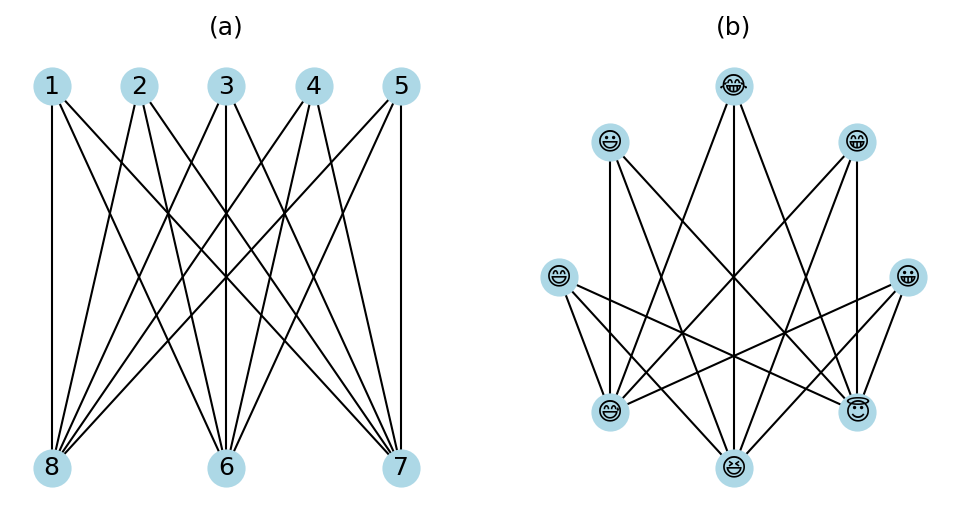
\includegraphics[scale=0.7]{figures/g-002.png}
    \caption{Both (a) and (b) are $K_{5,3}$.}
    \label{fig:2}
\end{figure}

\begin{proposition}
    Let $G[X, Y]$ and $H[U, V]$ be two complete bipartite graphs with $\abs{X} = \abs{U}$ and $\abs{Y} = \abs{V}$. Then $G \cong H$. In other words, a complete bipartite graph is unique up to isomorphism if the sizes of its two vertex sets in bipartition are determined.
\end{proposition}

\begin{proof}
    Since $\abs{X} = \abs{U}$ and $\abs{Y} = \abs{V}$, we can find a bijection $\theta: V(G) \to V(H)$ in such a way that $\theta$ maps each point in $X$ onto $U$, and each point in $Y$ onto $V$. Then for an edge $xy \in E(G)$, we have $\theta(x)\theta(y) \in E(H)$ since there has to be an edge connecting $\theta(x) \in U$ and $\theta(y) \in V$ by the definition of complete bipartite graphs. This proves $G \cong H$ by Proposition~\ref{pro:1}.
\end{proof}



%------------------------------

\section{Vertex Degrees}

%------------------------------





%------------------------------

\section{Paths and Connection}

\begin{proposition}
    If there is a $(u, v)$-walk in $G$, then there is also a $(u, v)$-path in $G$.
\end{proposition}

This can be proved easily using the following algorithm (Algorithm~\ref{alg:1}).

\begin{algorithm}[ht]
    \KwIn{A walk $W = v_0 e_1 v_1 \cdots e_k v_k$}
    \KwOut{A path $P$}
    initialize $P$ as a sequence containing just one vertex $v_0$ \;
    \For{$i = 1, \ldots, k$}{
        \eIf{$v_i$ is not in $P$}{
            append $e_i$ and $v_i$ to $P$ \;
        }{
            remove all the vertices and edges after the vertex $v_i$ from $P$ \;
        }
    }
    \caption{Extracting a Path From a Walk}
    \label{alg:1}
\end{algorithm}

%------------------------------

\begin{proposition}
    The number $(v_i, v_j)$-walks of length $k$ in $G$ is the $(i,j)$-th entry of the $k$-th power of the adjacency matrix $A$, i.e., $A^k$.
\end{proposition}

\begin{proof}
    % TODO
\end{proof}

%------------------------------

\section{Cycles}

%------------------------------

One simple yet useful observation of a particular longest path in a graph is that all the neighbors of the terminus must occur along the path. To be specific, if $P = v_0 e_1 v_1 \cdots e_k v_k$ is one of the longest paths in $G$ then $P$ must contain all vertices in $N(v_k)$. To prove this, we assume $P$ does not contain $v_{k+1} \in N(v_k)$. (Suppose $\psi(e_{k+1}) = v_k v_{k+1}$.) Then the path $P + e_{k+1}v_{k+1}$ is clearly longer than $P$, which leads to a contradiction. Figure~\ref{fig:1} depicts such an example. Note that if $8$ were a neighbor of $7$, then path $12345678$ would be longer.

\begin{figure}[ht]
    \centering
    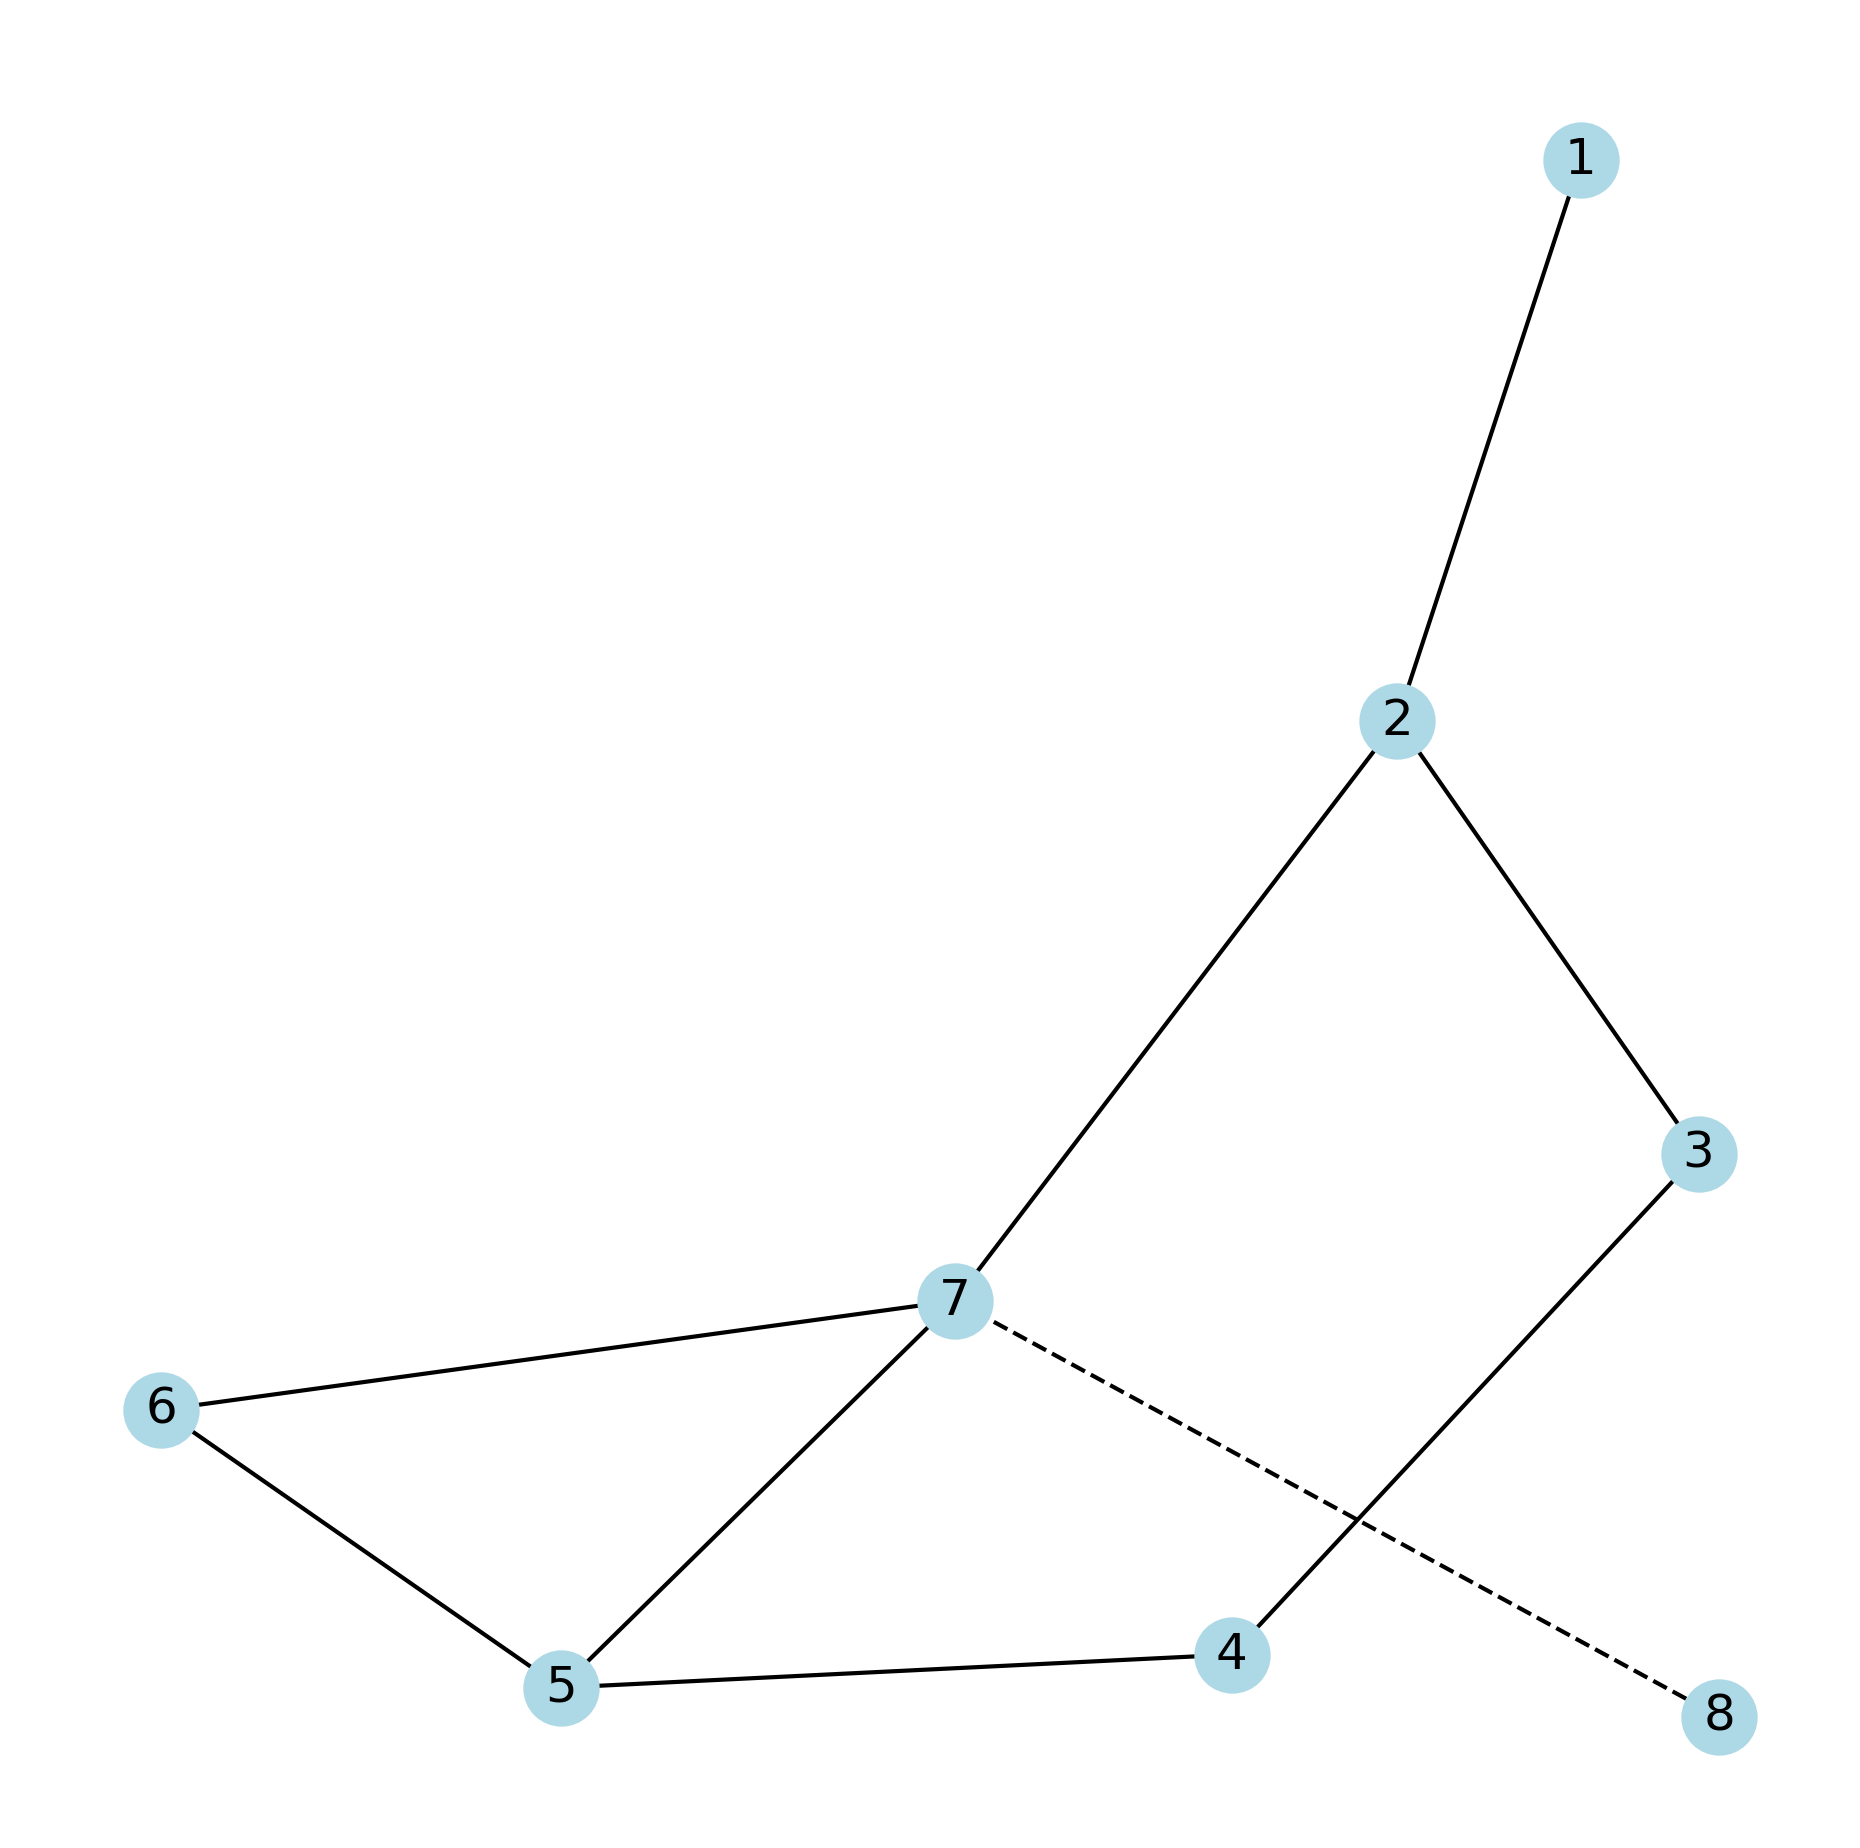
\includegraphics[scale=0.7]{figures/g-001.png}
    \caption{Path $1234567$ is one of the longest paths.}
    \label{fig:1}
\end{figure}

%------------------------------

\begin{proposition}
    If $\delta(G) \geq 2$, then we can find a cycle starting from each vertex of $G$.
\end{proposition}

\begin{proof}
    The conclusion is trivial if $G$ has a loop. Now, we assume that $G$ contains no loops. 
    \begin{note}
        Note that there are cases where $G$ has no paths if we allow it to have loops. For example, if every vertex of $G$ is incident with just exactly one loop, then $G$ still satisfies the hypothesis. But there are no paths in $G$.
    \end{note}
    \noindent Let $P = v_0 e_1 v_1 \cdots e_{k-1} v_{k-1} e_k v_k$ be one of the longest paths in $G$. Since $\deg(v_k) \geq 2$ and $v_k$ has no loops, $v_k$ has a neighbor, say $u$, other than $v_{k-1}$. As noted before, $u$ must occur in $P$. Therefore, there exists a cycle from $u$ to $u$.
\end{proof}

In fact, we have an algorithm to find a cycle without knowing the longest path in $G$.

\begin{algorithm}[ht]
    \KwIn{$G$ with $\delta(G) \geq 2$}
    \KwOut{A cycle $C$}
    \If{$G$ has a loop $e$ from $v$ to $v$}{
        $C \gets v e v$ \;
        \Return{$C$} \;
    }
    pick a vertex $v_0$ \; 
    $P \gets v_0$ \;
    pick $v \in N(v_0)$ and let $e$ be the corresponding edge, i.e., $\psi(e) = v_0 v$ \;
    \While{$v$ is not in $P$}{
        $P \gets P + e v$ \;
        pick $u \in N(v)$ such that
        there exists an edge $f$ satisfying $\psi(f) = v u$ and $f \neq e$ \;
        $v \gets u$ \; 
        $e \gets f$ \;
    }
    remove from $P$ all vertices and edges before $v$ \;
    $C \gets P + ev$ \;
    \caption{Finding a Cycle in $G$ With $\delta(G) \geq 2$}
    \label{alg:2}
\end{algorithm}

\begin{proof}
    We need to show that Algorithm~\ref{alg:2} works correctly. 
    
    (initialization) Firstly, note that line 7 is possible since $v_0$ has no loops and $\deg(v_0) \geq 2$. 

    We claim the loop invariants are
    \begin{enumerate}
        \item $P$ has $j$ vertices assuming that we are to execute the $j$-th iteration,
        \item $P$ has no duplicated vertices, i.e., $P$ is a path, and
        \item edge $e$ is incident with $v$.
    \end{enumerate}

    (Maintenance) Suppose we are in the $j$-th iteration. After line 9, $P$ remains a path. Because $\deg(v) \geq 2$, there exists an edge $f$ other than $e$ that is incident with $v$. Hence, line 10 works correctly.  After executing line 12, we find that the number of vertices in $P$ is increased by one, i.e., $j+1$, $P$ is still a path and $e$ is incident with $v$.

    (Termination) We can complete at most $n-1$ iterations since $P$ can hold at most as many vertices as there are in $G$. Upon termination, we find $v$ is in $P$ and $e$ is incident with $v$. By removing from $P$ all vertices and edges before $v$ and then append to it edge $e$ and vertex $v$, we will obtain a cycle from $v$ to $v$. 
\end{proof}

%==============================

% references
\printbibliography[heading=bibintoc, title=References]

%==============================

% print index page
\printindex

%==============================

\end{document}